\section{Frontend}\label{5_4_software}
\subsection{Unity3D and Kinect SDK}
% KinectStudio, VGB, Unity3D, Kinect SDK for unity, Kinect MS-SDK
The software development process consists of the interplay of two major software components (Figure~\ref{fig:5_3_unityKinectArchitecture}).
First the cross-platform game engine \textit{Unity3D} by \textit{Unity Technologies}. It is widely known for game development but also for development with several interaction devices (e.g. \textit{HTC Vive}, \textit{Leap Motion}). Applications can be deployed for various platforms like desktop, mobile, web, console, TV, or virtual/augmented/mixed reality devices.
Unity is used in the SLS to create the virtual environment, interface design, manage actions by the user, and for data management.
%(e.g. Windows, macOS, Android, iOS, Oculus Rift, Windows Mixed Reality and so on).
\begin{figure}[htb]
	\centering
	\begin{minipage}[t]{1\linewidth}
		\centering
		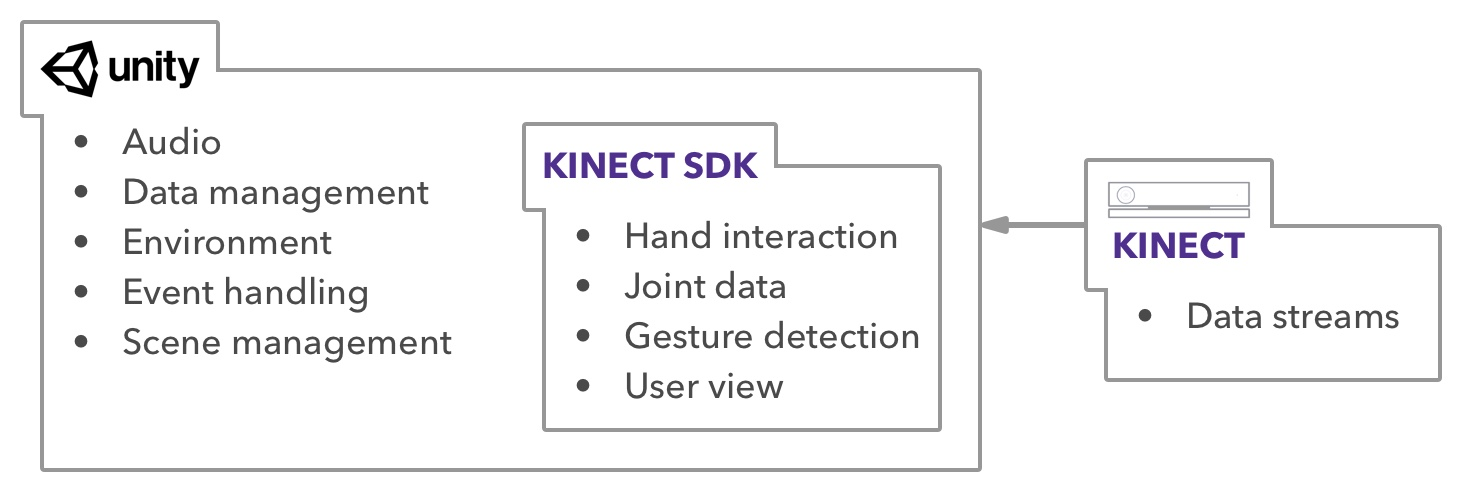
\includegraphics[width=1\linewidth]{Pictures/5_3_unityKinectArchitecture}
		\caption{Unity and Kinect architecture}%
		\label{fig:5_3_unityKinectArchitecture}
	\end{minipage}
\end{figure}

As second component the \textit{Microsoft Kinect SDK v2.0}~\footnote{\label{fn:kinectTools}\url{https://developer.microsoft.com/de-de/windows/kinect/tools}} has to be installed on the PC as well.
It consists of several tools, application examples, and scripts to access the data stream of the Kinect.
Microsoft offers also a \textit{Kinect for Windows Unity package}\cref{fn:kinectTools} to create a Kinect based Unity application.
%Since \textit{Unity 5} it can be used with the free personal edition of Unity, whereas before it could be only used with the pro version.
The \textit{Kinect v2 Examples with MS-SDK} \footnote{\url{https://www.assetstore.unity3d.com/en/\#!/content/18708}} package by Rumen Filkov was used to get an idea on how to handle the data streams of the Kinect.
In addition it makes accessing input data of the user recognized by the Kinect, like e.g. joint position and interaction implementation, more simple and provides several code examples.

%make data access and interaction implementation more simple as well as 
%The plugin is used for accessing input data of the user recognized by the Kinect device like e.g. joint position, gesture detection, and user actions.

%The JSON datafiles can be easily accessed in Unity via the JSON serialization feature~\footnote{\url{https://docs.unity3d.com/Manual/JSONSerialization.html}}. \todo{1-2 sätze mehr dazu}

\subsection{Implementation}
The frontend implementation of the SLS will be explained on the basis of the workflow that a user would run through. It consists of four main parts. First a small tutorial to get familiar with the interaction,  second the selection menus, third the description and introduction of a level as well as an exercise, and fourth the exercise execution with real-time feedback. 
%interaction integration, and feedback implementation of the system are further described.

\subsubsection{Interaction Tutorial}
If a user starts with the SLS (Figure~\ref{fig:5_3_welcome}) an engagement gesture is the very first interaction. She has to raise any hand over the head. This conveys that the system recognises and reacts to specific movement actions. 

Afterwards the user is introduced into the interaction techniques (Figure~\ref{fig:5_3_tutHandPush} \&~\ref{fig:5_3_tutHandPoint} ).
Her hands serve hereby as input for navigating and interacting with interface elements in the SLS. Therefore she is in constant interaction with the system and becomes more familiar to it.
The current position on the screen is visualised by a virtual hand cursor.

\begin{figure}[htb]
	\centering
	\begin{minipage}[t]{0.32\linewidth}
		\centering
		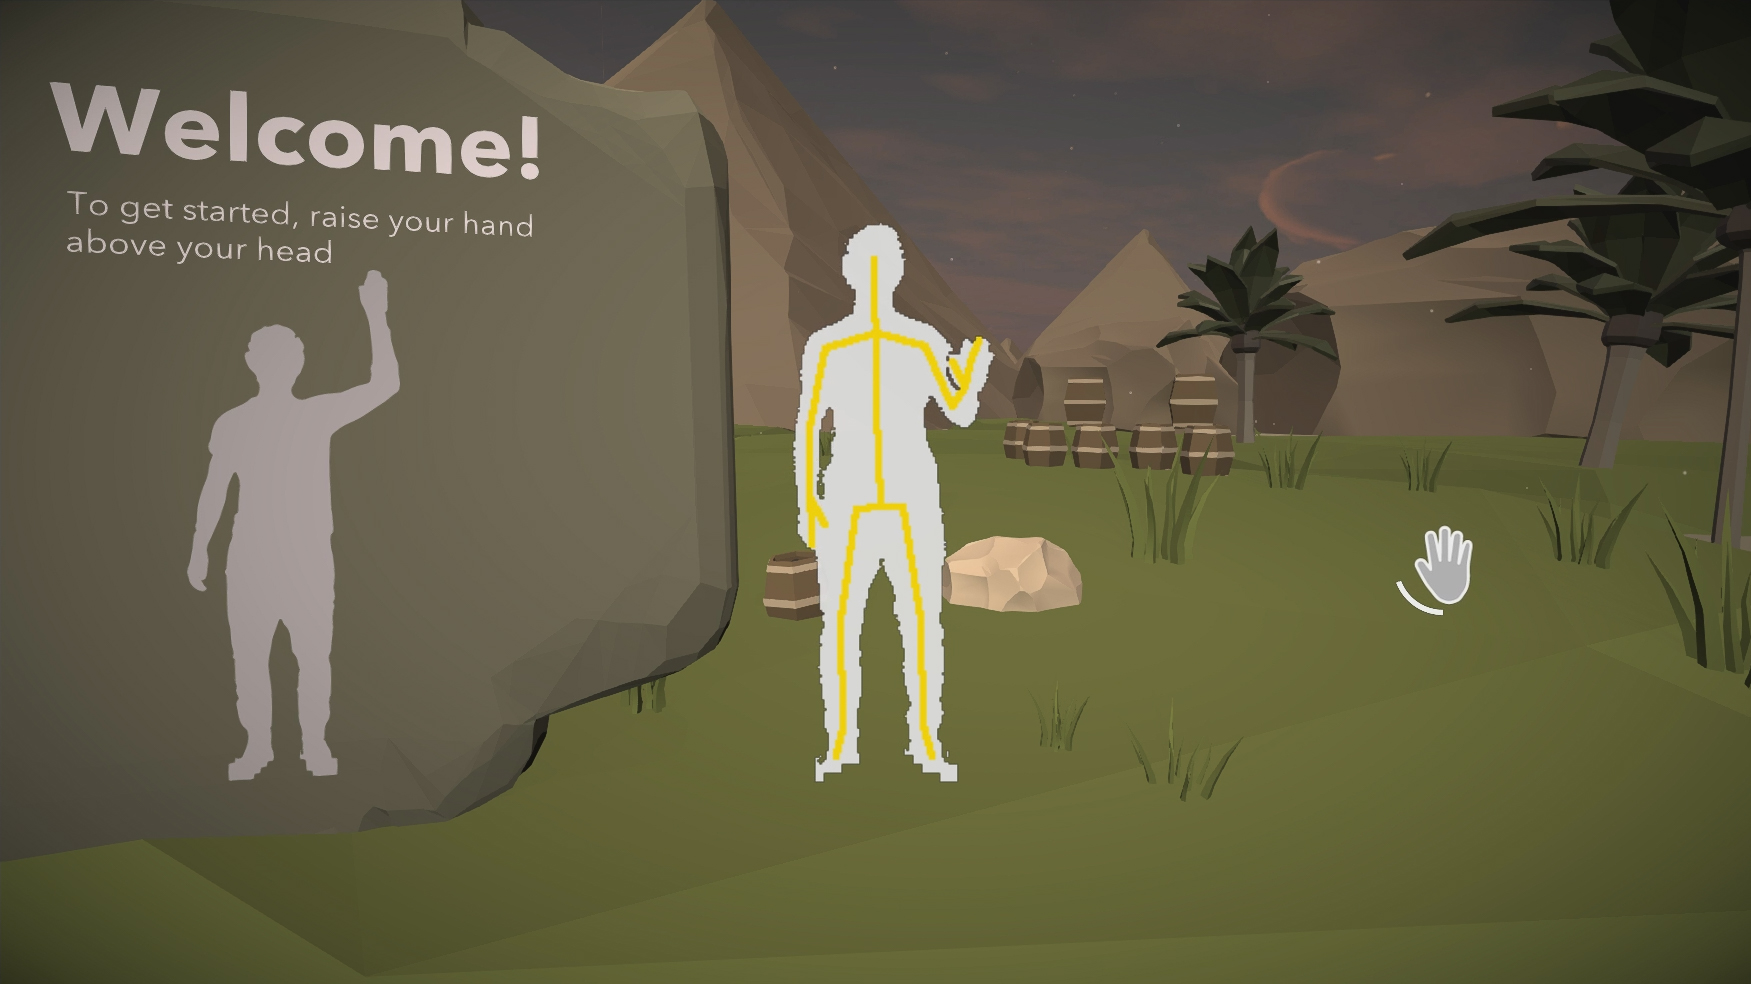
\includegraphics[width=1\linewidth]{Pictures/5_Workflow/1_Welcome}
		\subcaption{Welcome screen with engagement gesture}
		\label{fig:5_3_welcome}
	\end{minipage}
	\hfill
	\begin{minipage}[t]{0.32\linewidth}
		\centering
		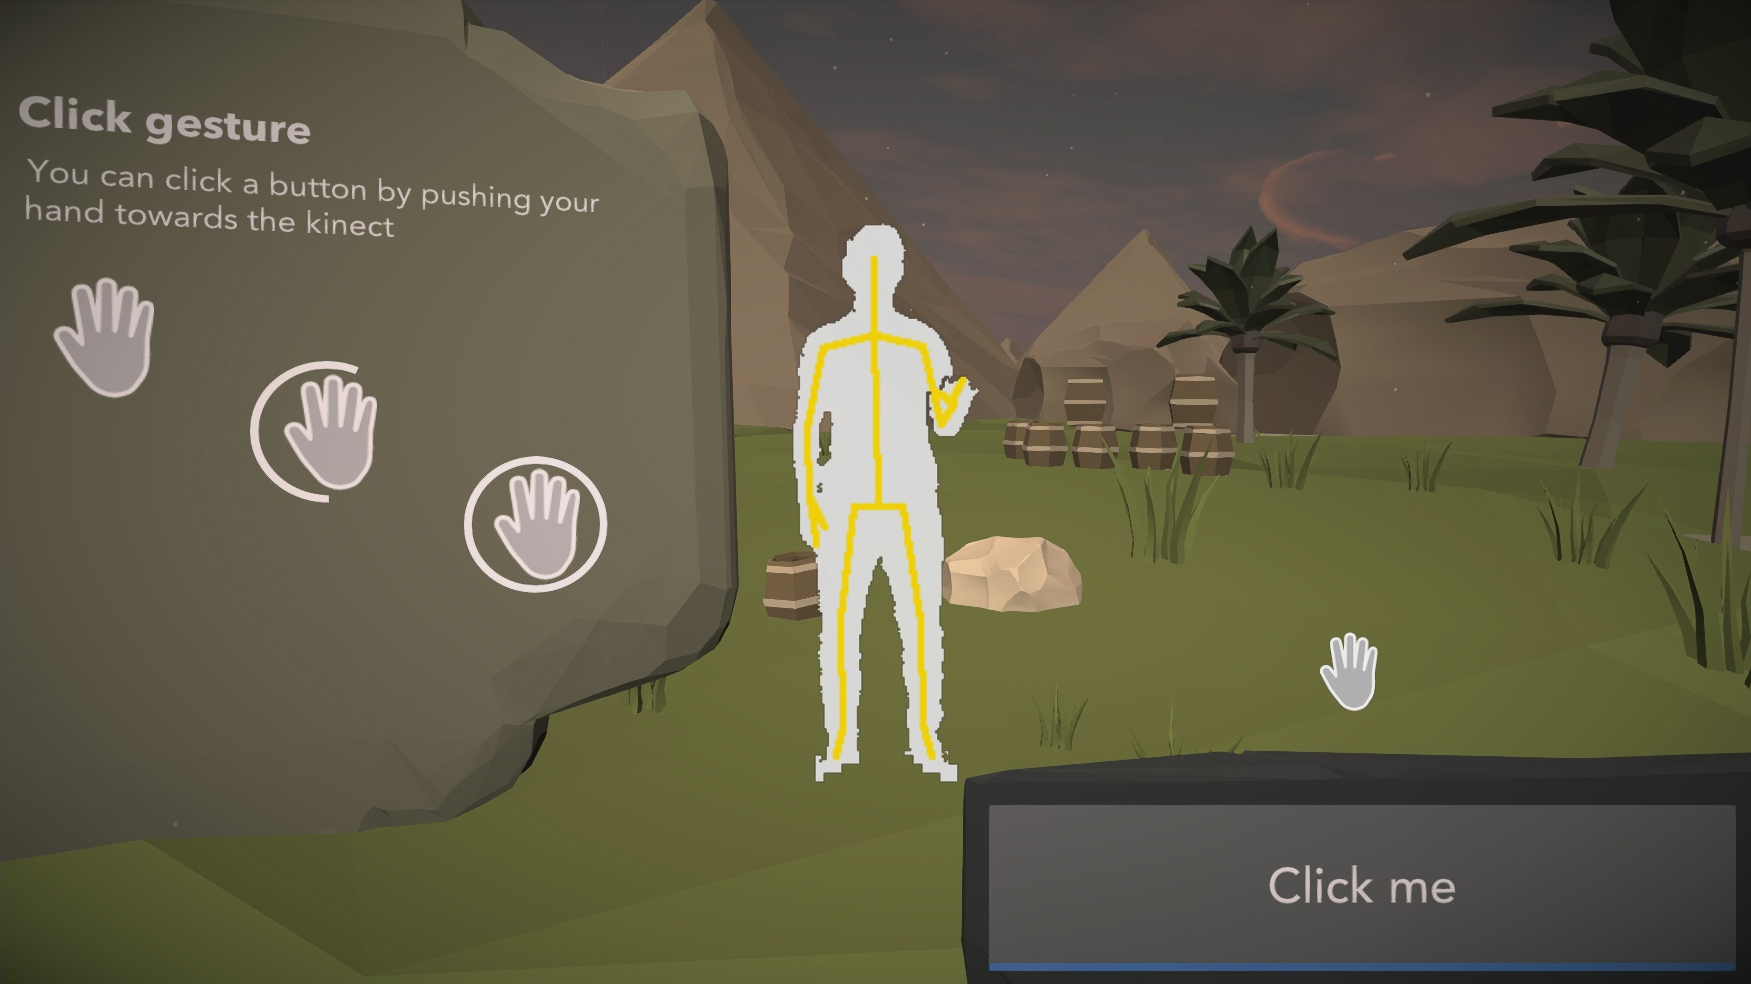
\includegraphics[width=1\linewidth]{Pictures/5_Workflow/2_TutHandPush}
		\subcaption{How to click part I}
		\label{fig:5_3_tutHandPush}
	\end{minipage}
	\hfill
	\begin{minipage}[t]{0.32\linewidth}
		\centering
		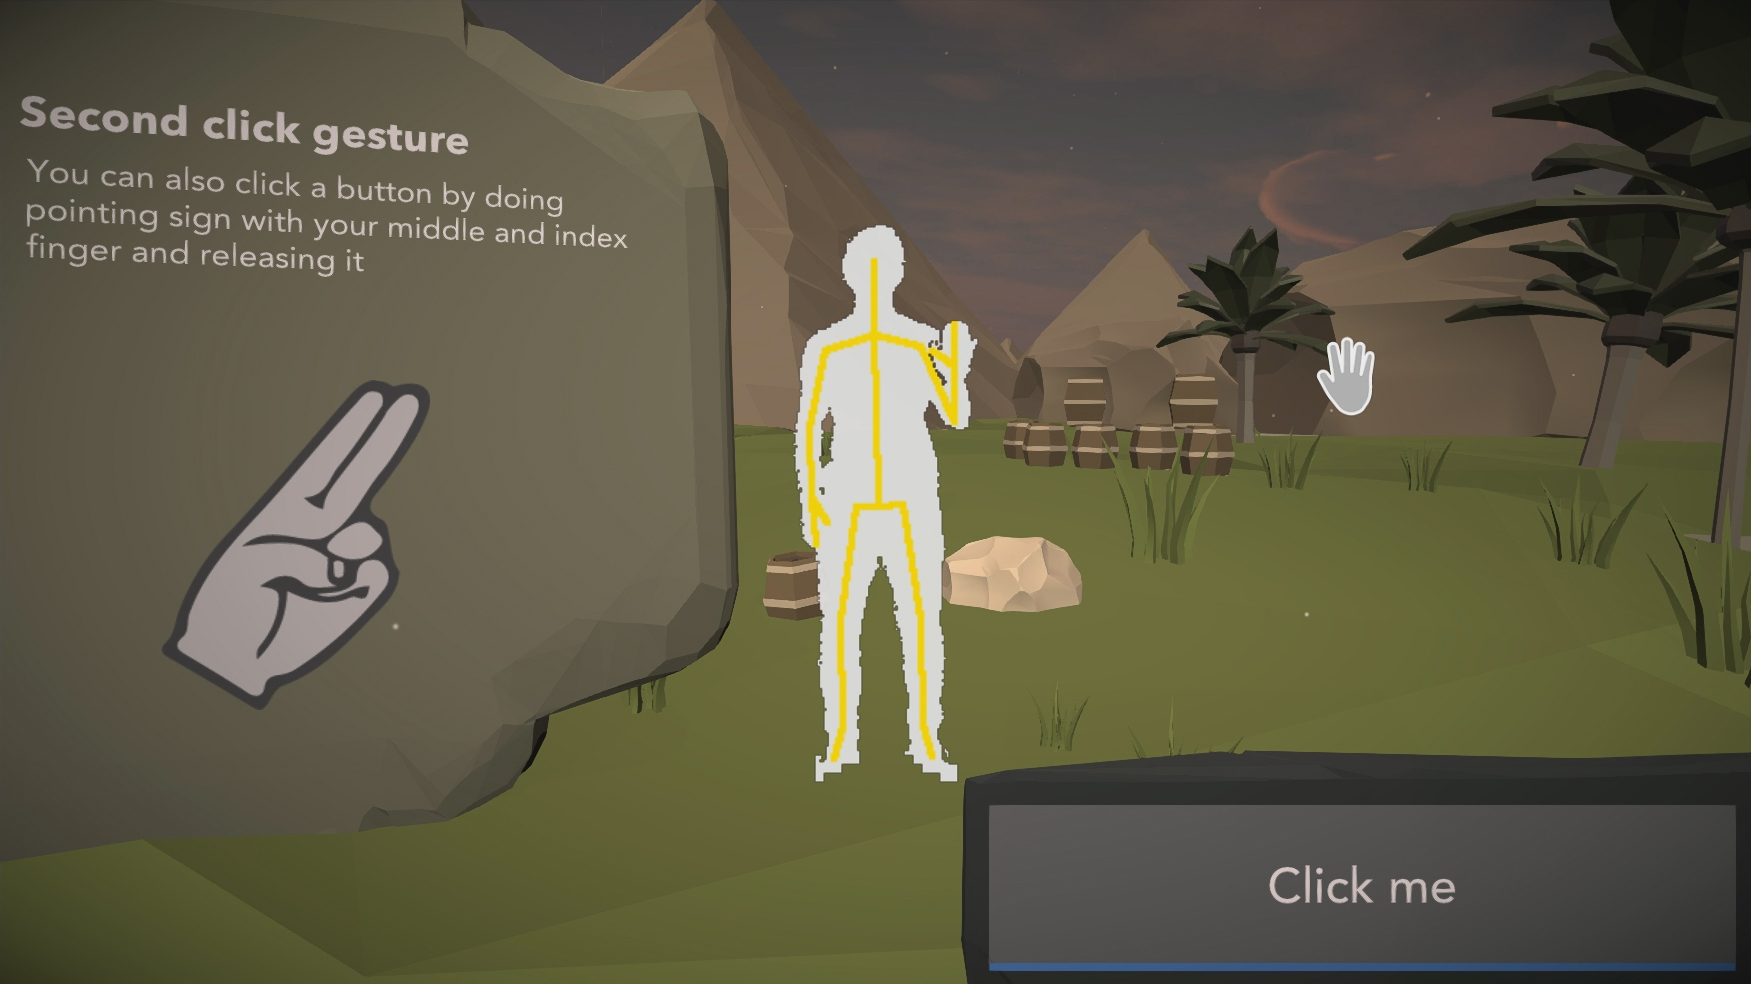
\includegraphics[width=1\linewidth]{Pictures/5_Workflow/3_TutHandClick}
		\subcaption{How to click part II}
		\label{fig:5_3_tutHandPoint}
	\end{minipage}
	\caption{Instruction on how to use the SLS}
	\label{fig:5_3_tutorials}
\end{figure}
%She has to raise her hand over the head whereupon the system conveys that it recognises specific user actions.

%A code example on how to this gesture is implemented can be seen in listing~\ref{lst:codeEngagement}.

%The \textit{KinectManager} exists as an empty \textit{GameObject} in the scene and has to be referenced in the script. The \textit{KienctInterop} class delivers several utility and interop function and calls the sensor interfaces. Here it is used to assign the proper joint type for tracking them. 
%First the developer has to assure that the Kinect is initialized, a user has been detected, and the relating joints are recognized. A condition checks if the current vertical position of the right hand is above the head joint (\textit{Listin~\ref{lst:codeEngagement} line~\ref{lst:codeEngagement15}}). If this is the case, the next scene can be loaded. 
%This is actually part of the script for the first scene in the application, in which the user has to engage with the Kinect by doing the described movement.

% provide the possibility of an autonomous interaction the user has to navigate on her own with the system.
%Her hands serve as input for interacting with interface elements.

Four different approaches were tested as hand interaction gesture.
First, hovering with the hand over elements for a few seconds (Figure~\ref{fig:5_3_hover}).
It caused problems because of accidental and unwanted misclicks due to relatively big and many interaction elements in the interface.
As second interaction technique the hand should be closed to a fist or grab gesture (Figure~\ref{fig:5_3_fist}).
It also triggered unwanted misclicks if the hand of the user closes a bit during navigation.
%The hand of the users closes automatically a little bit during the interaction, which in combination with the standing position on the outermost tracking range was sufficient to trigger a click.%(Figure \todo{comparison default \& target})
A better interaction was performed by the so called \textit{V-sign}, where the user makes a pointing gesture with her index and middle finger.
The click event triggers when the user releases her hand into the default state (Figure~\ref{fig:5_3_point}).
Relating to the real word, a button is triggered by pushing it down with the hand or finger.
This is used as an analogy in the last interaction gesture, where the user pushes the open hand towards the Kinect.
It is the most intuitive, natural, and least error-prone technique (Figure~\ref{fig:5_3_push}). %Since in this gesture the hand has to move from point a to point b in the z-axis the progress is visualized by a filling circle like seen in figure~\ref{fig:handcursorProgress}.
Therefore the push technique is used as main interaction. The V-sign is implemented as second interaction technique, since it resulted in better interaction experience than the fist and hover gesture.
\begin{figure}[htb]
	\centering
	\subcaptionbox{Hover and wait\label{fig:5_3_hover}}
		[0.24\linewidth]{
\includegraphics[width=0.12\linewidth]{Pictures/5_3_hover}}
	\subcaptionbox{Grab/Fist\label{fig:5_3_fist}}%
		[0.24\linewidth]{
\includegraphics[width=0.08\linewidth]{Pictures/5_3_fist}}
	\subcaptionbox{Pointing\label{fig:5_3_point}}%
		[0.24\linewidth]{
\includegraphics[width=0.097\linewidth]{Pictures/5_3_point}}
	\subcaptionbox{Pushing hand\label{fig:5_3_push}}%
		[0.24\linewidth]{
\includegraphics[width=0.176\linewidth]{Pictures/5_3_push2}}
	\caption{Several tested hand interaction techniques}%
	\label{fig:5_3_handInteraction}
\end{figure}

When finished with the interaction techniques the user is introduced on how to stand in the right starting position (Figure~\ref{fig:5_3_standingPosition}). She has to stand with both feet parallel and in front to the Kinect. This ensures the readiness of the user and is required before starting the exercise execution.
%Furthermore the initial joint positions of the foot is taken to verify if the user stands on the ground or on the line during the appropriate exercises.
%This initial joint position can differ if the user stands closer or more far away from the sensor because of the Kinects angel regarding its height. Hence the z-axis joint position of the left and right feet will be compared to have the same value with a little tolerance. 
\begin{figure}[htb]
	\centering
	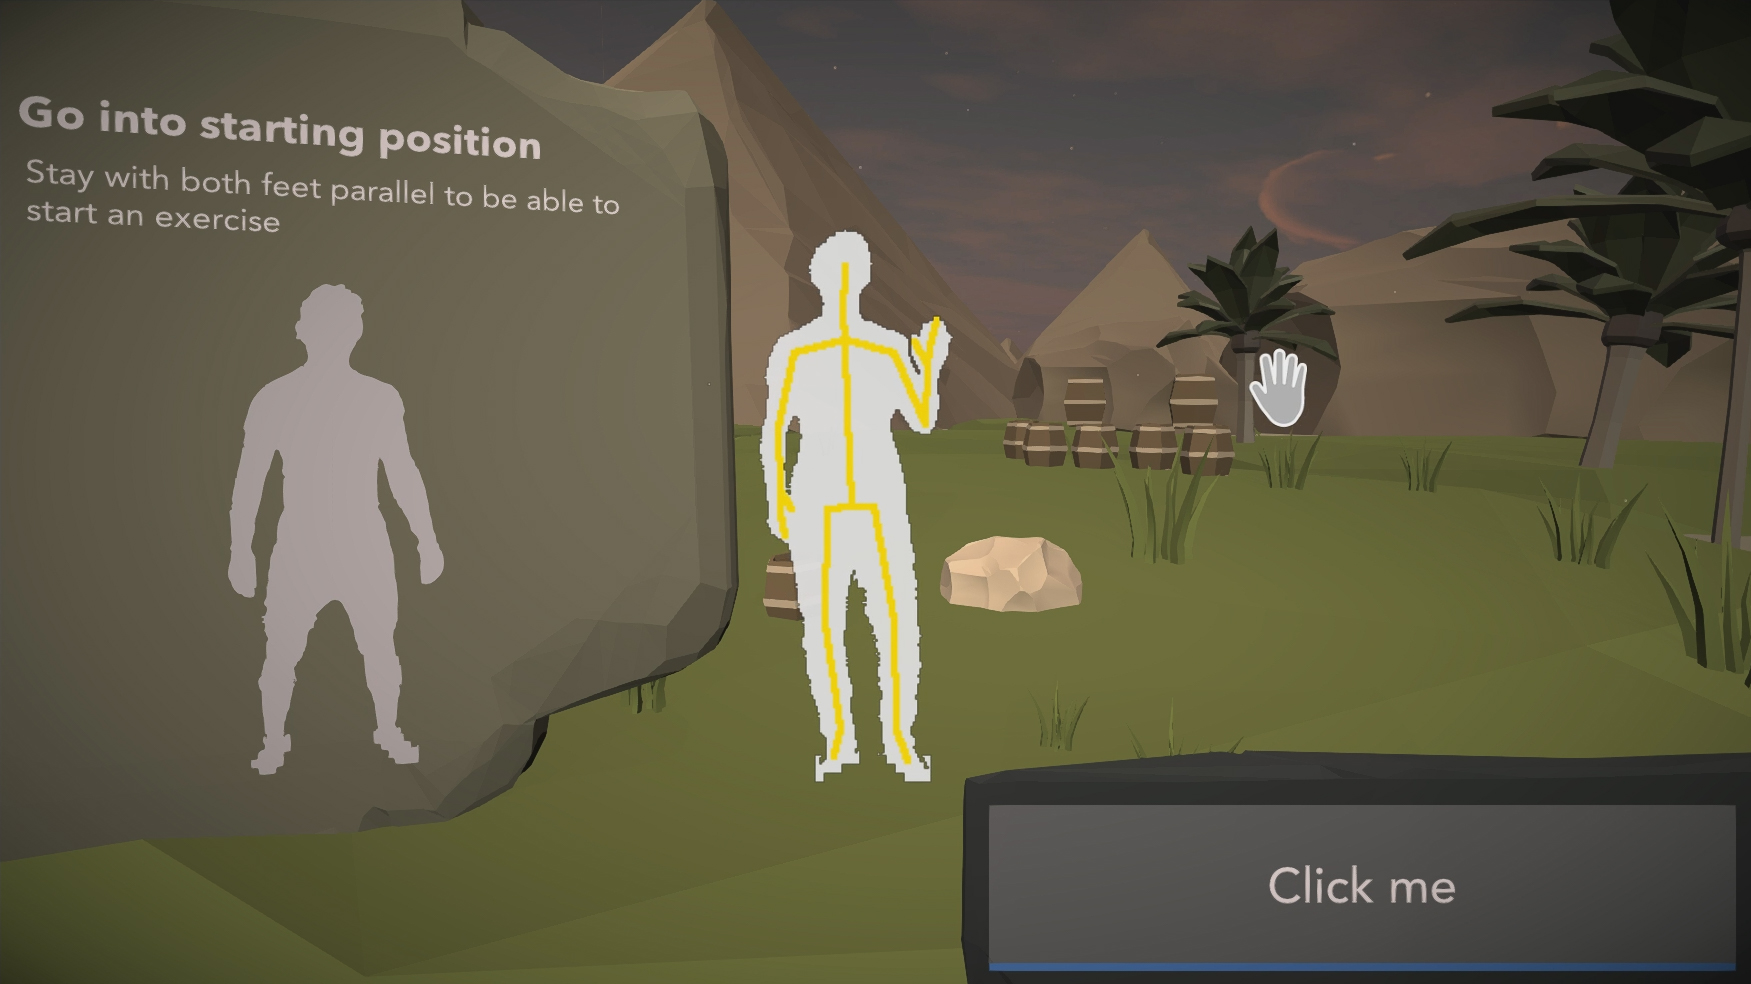
\includegraphics[width=0.5\linewidth]{Pictures/5_Workflow/4_2_StartingPosition}
	\caption{Instruction on how to use stand in the correct position}
	\label{fig:5_3_standingPosition}
\end{figure}

\subsubsection{Selection Menus}
The system consists of several selection menus. At first a user profile has to be selected (Figure~\ref{fig:5_3_user_menu}). Hereby it provides the possibility that more than one user can train with the system separately.
%When the trainee selects her profile the system checks if the JSON file has any data. If no data is available, which means it is a new user, the default exercise JSON file will be copied into the profile. 
When selecting a profile the appropriate JSON file will be loaded into the system for accessing and managing the user data.
%The trainee selects her profile by herself. With this the data will be loaded into the system. In the user selection the trainee should select the right profile by herself to cover the condition of multiple user that can train with the system. 
%The users name and id are saved in as \textit{PlayerPrefs}. This is a class in Unity that provides the possibility to be globally accessible in the application. The respective code for setting and getting the values can be seen in listing \todo{ref listing playerpfrefs}. This is needed to find the correct path for the JSON files to save the data.

Levels and exercises are also structured as menu (Figure~\ref{fig:5_3_level_menu} \&~\ref{fig:5_3_exercise_menu}).
At first they are all locked except the very first one to provide a starting point.
A level can be unlocked by accomplishing each exercise of the previous level.
This procedure applies similarly to the exercises.
Hereby, the next exercise can be unlocked by accomplishing all body sides and repetitions of the current exercise.
%The structure already seen in section \textit{\ref{4_4_exercises}} is adapted to store the corresponding information for the tier, exercise, side, and repetition.
\begin{figure}[htb]
	\centering
	\begin{minipage}[t]{0.32\linewidth}
		\centering
		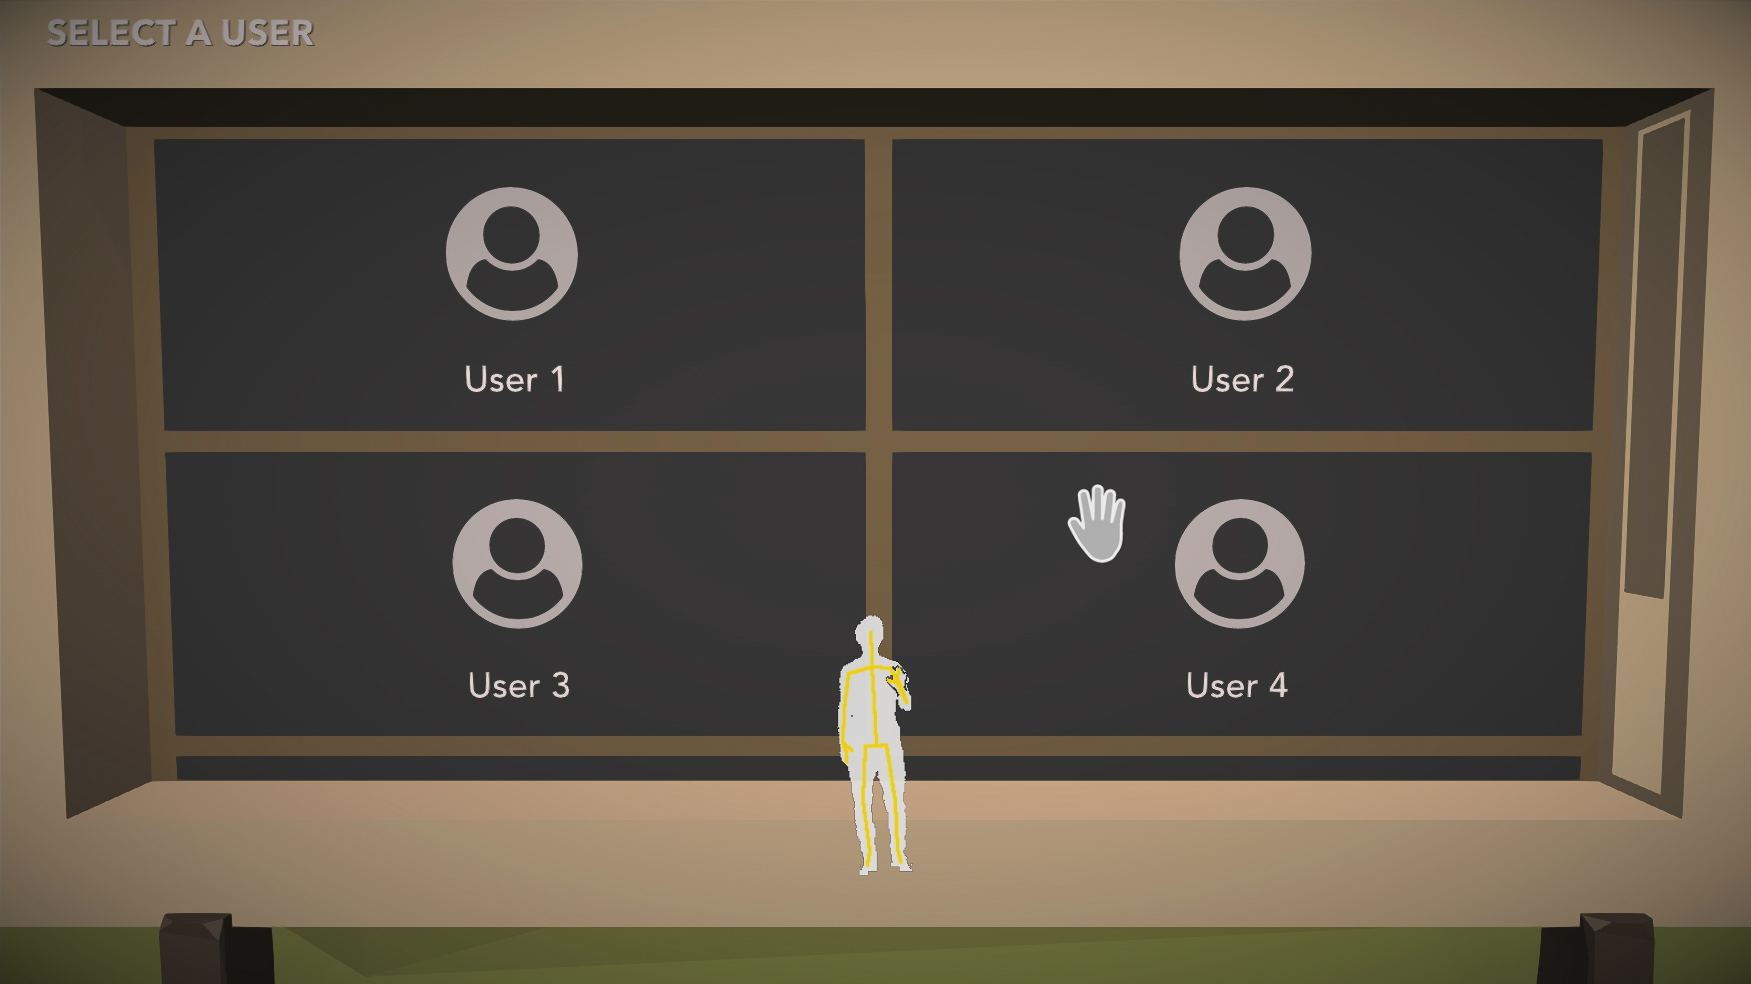
\includegraphics[width=1\linewidth]{Pictures/5_Workflow/5_UserMenu}
		\subcaption{User menu}%
		\label{fig:5_3_user_menu}
	\end{minipage}
	\hfill
	\begin{minipage}[t]{0.32\linewidth}
		\centering
		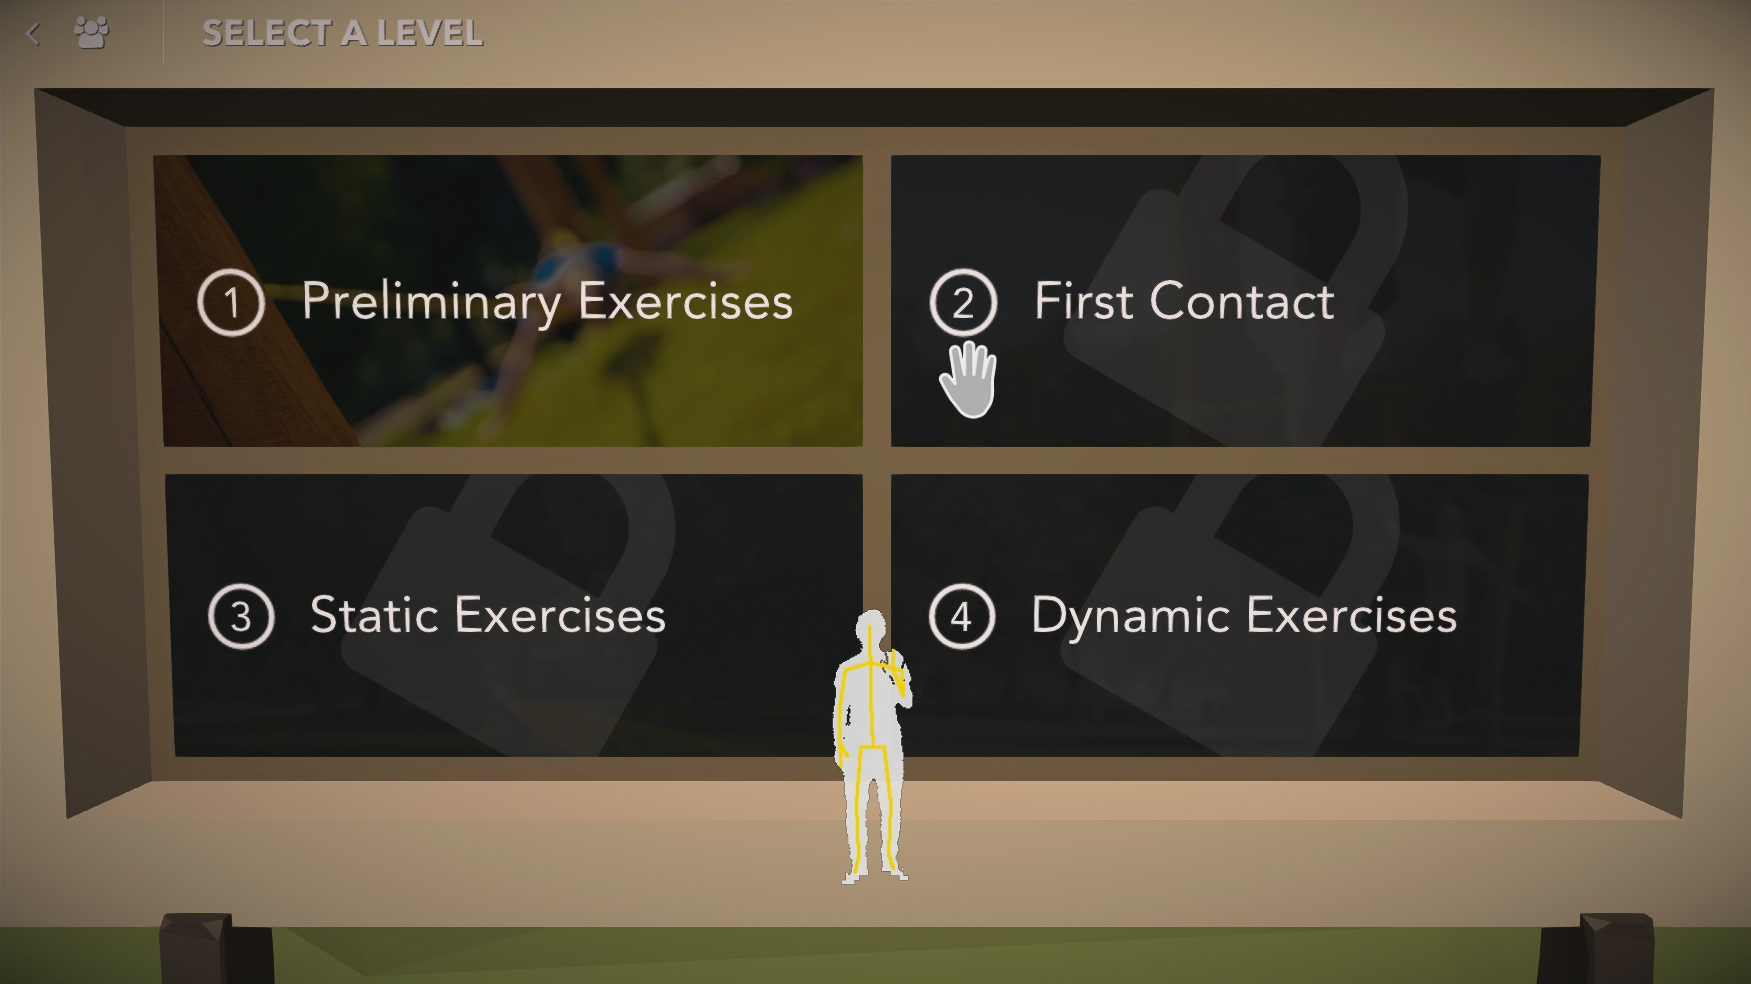
\includegraphics[width=1\linewidth]{Pictures/5_Workflow/6_LevelMenu}
		\subcaption{Level menu}%
		\label{fig:5_3_level_menu}
	\end{minipage}
	\hfill
	\begin{minipage}[t]{0.32\linewidth}
		\centering
		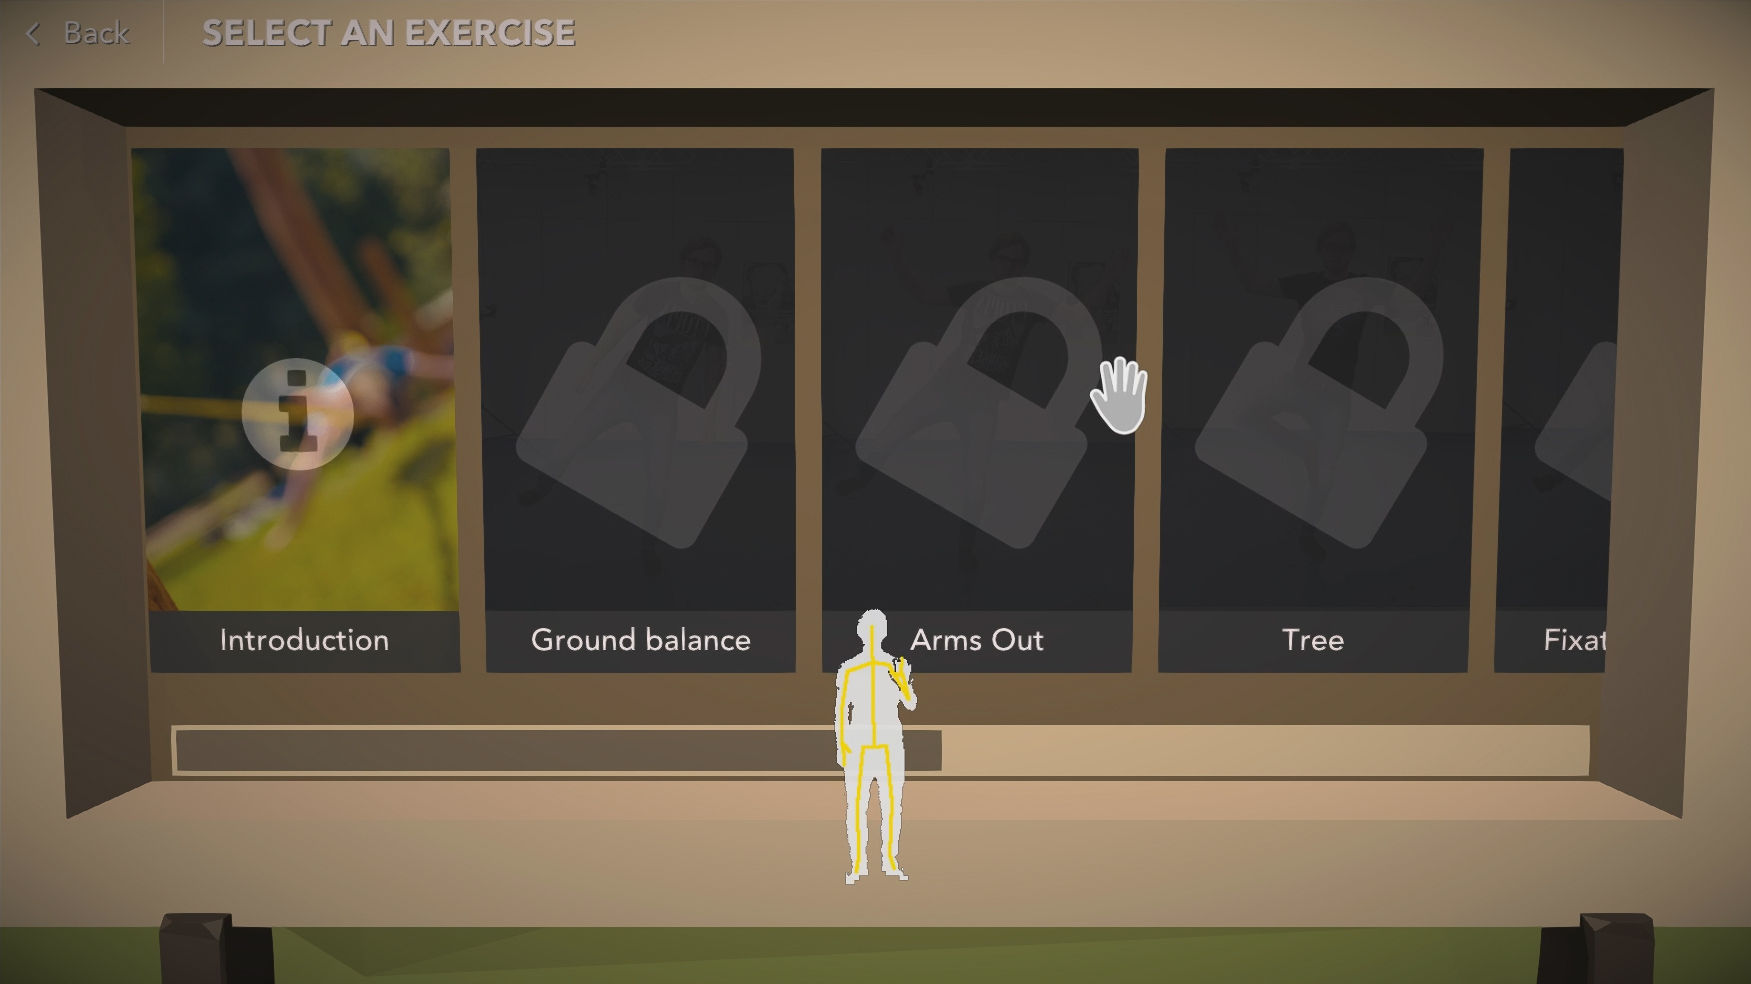
\includegraphics[width=1\linewidth]{Pictures/5_Workflow/7_1_ExerciseMenu}
		\subcaption{Exercise menu}%
		\label{fig:5_3_exercise_menu}
	\end{minipage}
	\caption{Visualisation of selection menus}%
	\label{fig:5_3_selection_menus}
\end{figure}

\subsubsection{Level and Exercise Description}
Selecting a level leads the user to the level introduction (Figure~\ref{fig:5_3_level_intro}). She is informed about the goals of the current level and gets helpful information for the execution of the following exercises. After that she selects the first exercise in the menu and afterwards a body side, which she wants to train first (Figure~\ref{fig:5_3_select_side}). This leads her to the detailed exercise description (Figure~\ref{fig:5_3_exercise_intro}). It is introduced by a list of actions she has to follow to perform it correctly. Additionally, the amount of repetitions and the minimum time to hold the gesture are given. Furthermore, a looping video on the visualizes the correct execution to the user.
\begin{figure}[htb]
	\centering
	\begin{minipage}[t]{0.32\linewidth}
		\centering
		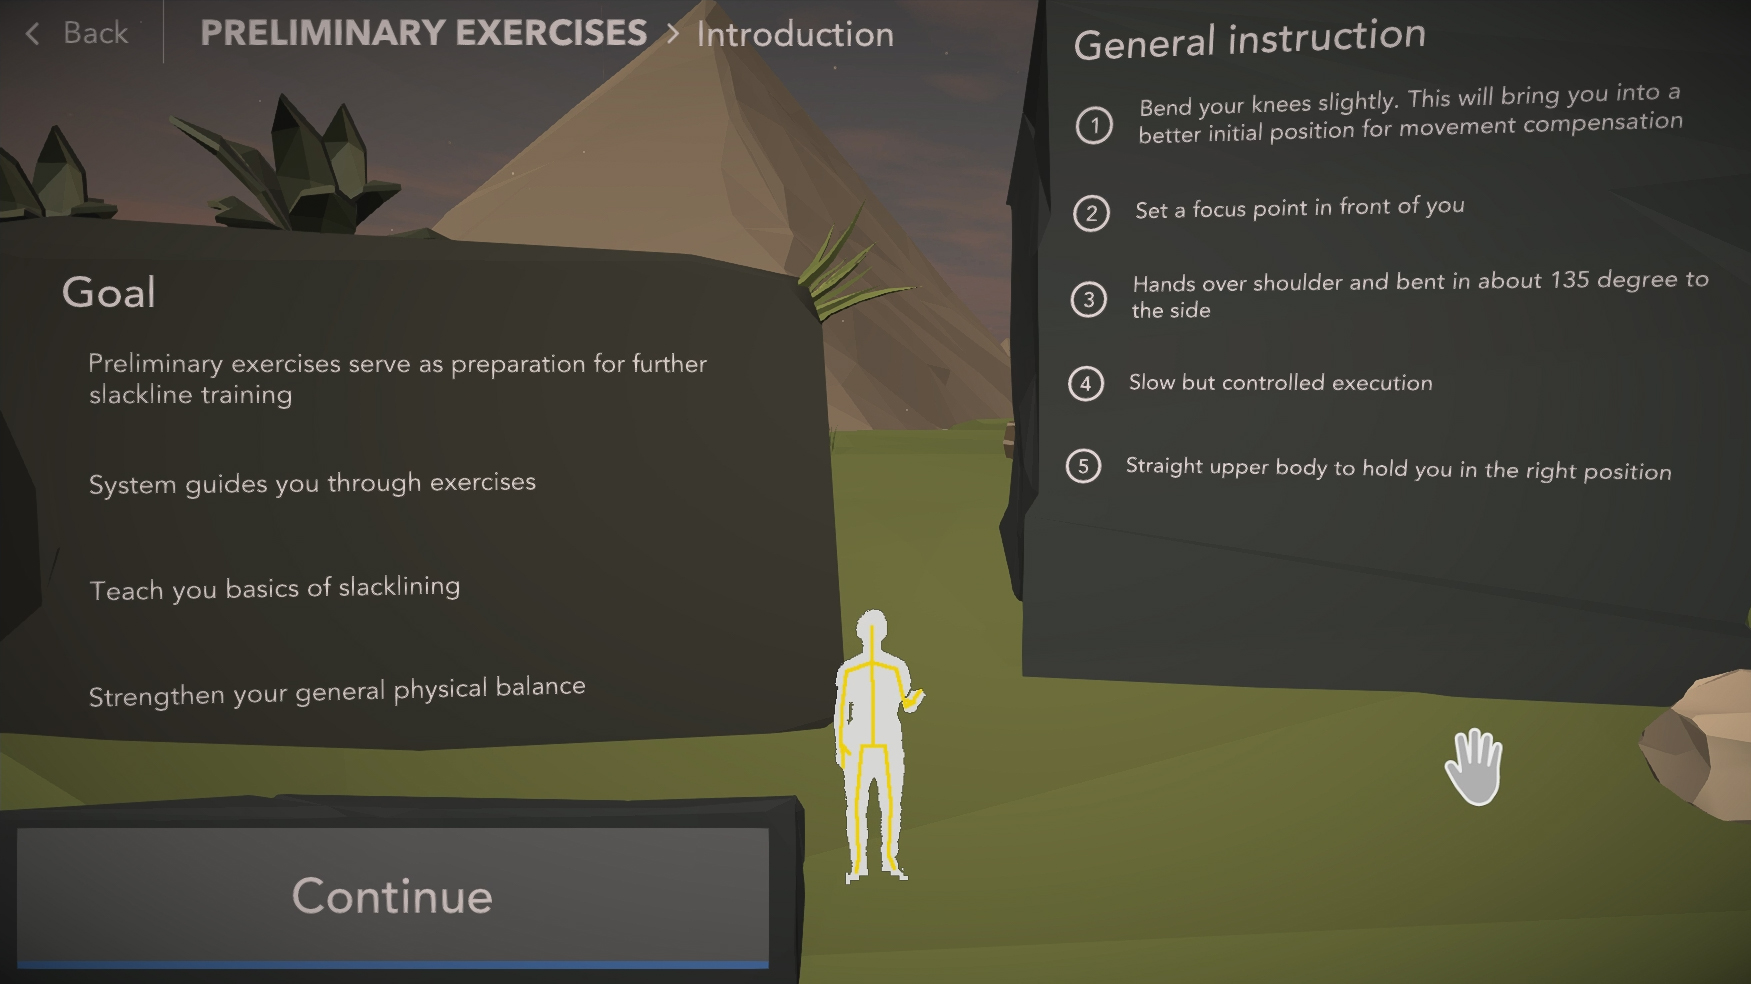
\includegraphics[width=1\linewidth]{Pictures/5_Workflow/8_LevelDescription}
		\subcaption{Goals \& tips for a level}%
		\label{fig:5_3_level_intro}
	\end{minipage}
	\hfill
	\begin{minipage}[t]{0.32\linewidth}
		\centering
		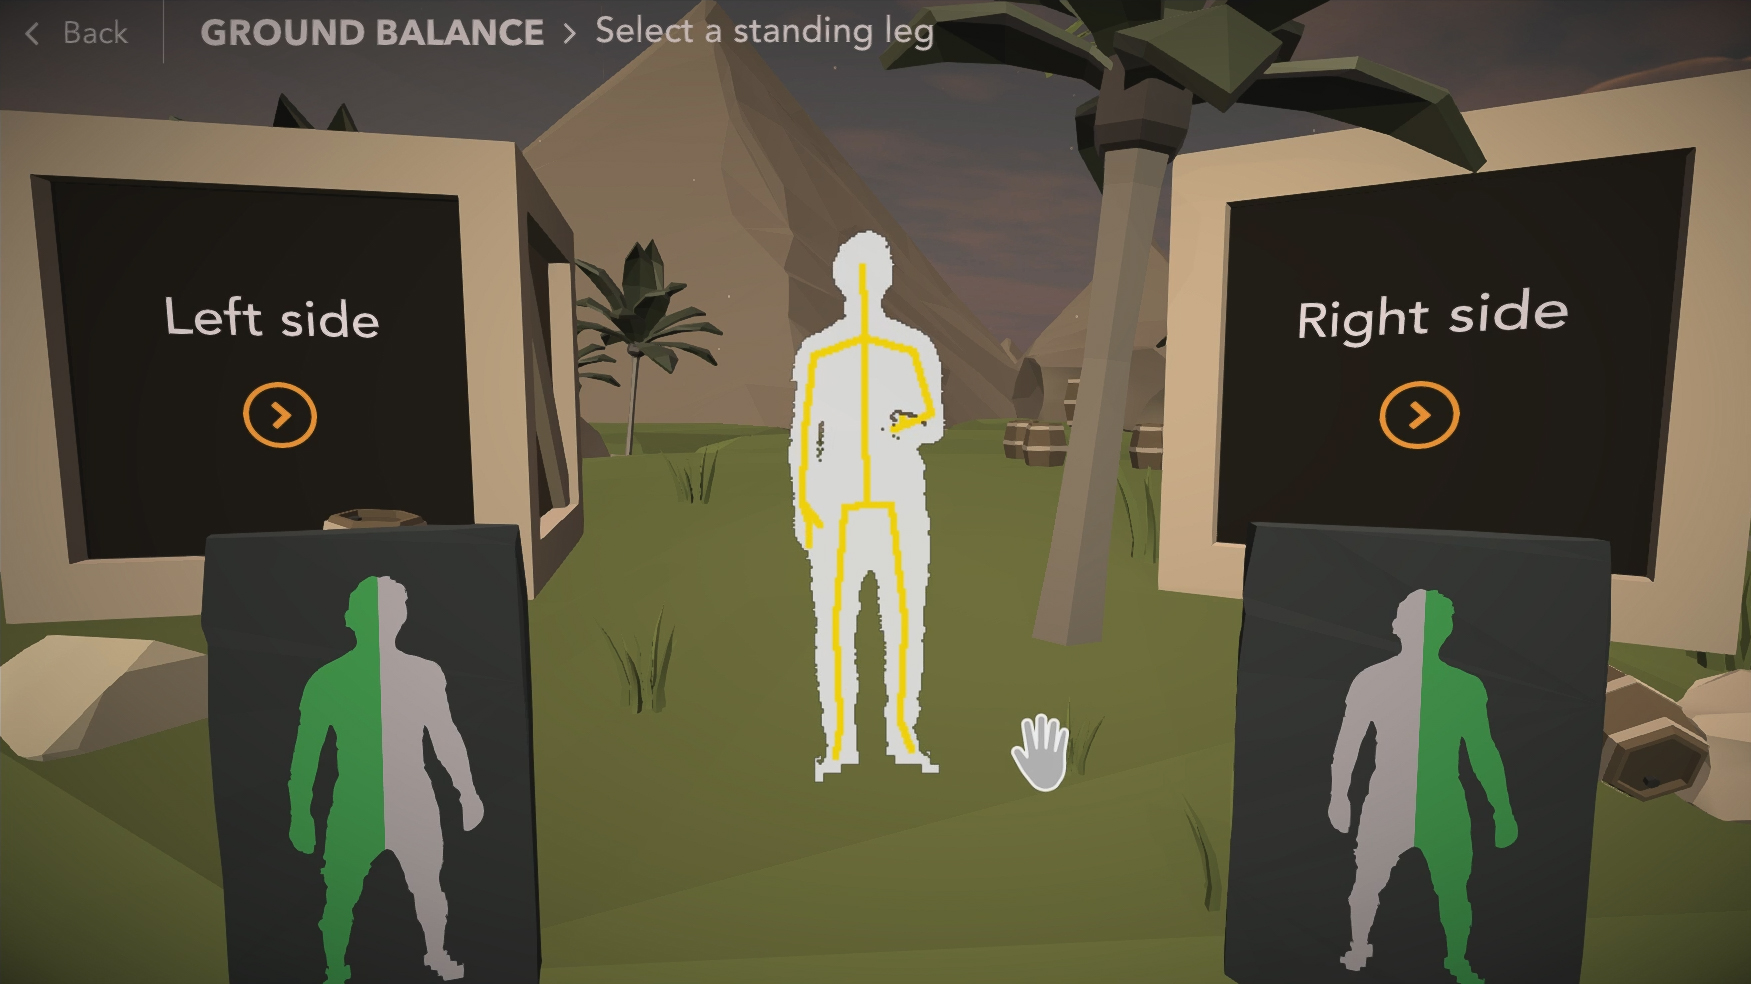
\includegraphics[width=1\linewidth]{Pictures/5_Workflow/9_1_SideSelectionNone}
		\subcaption{Selection of a body side}%
		\label{fig:5_3_select_side}
	\end{minipage}
	\hfill
	\begin{minipage}[t]{0.32\linewidth}
		\centering
		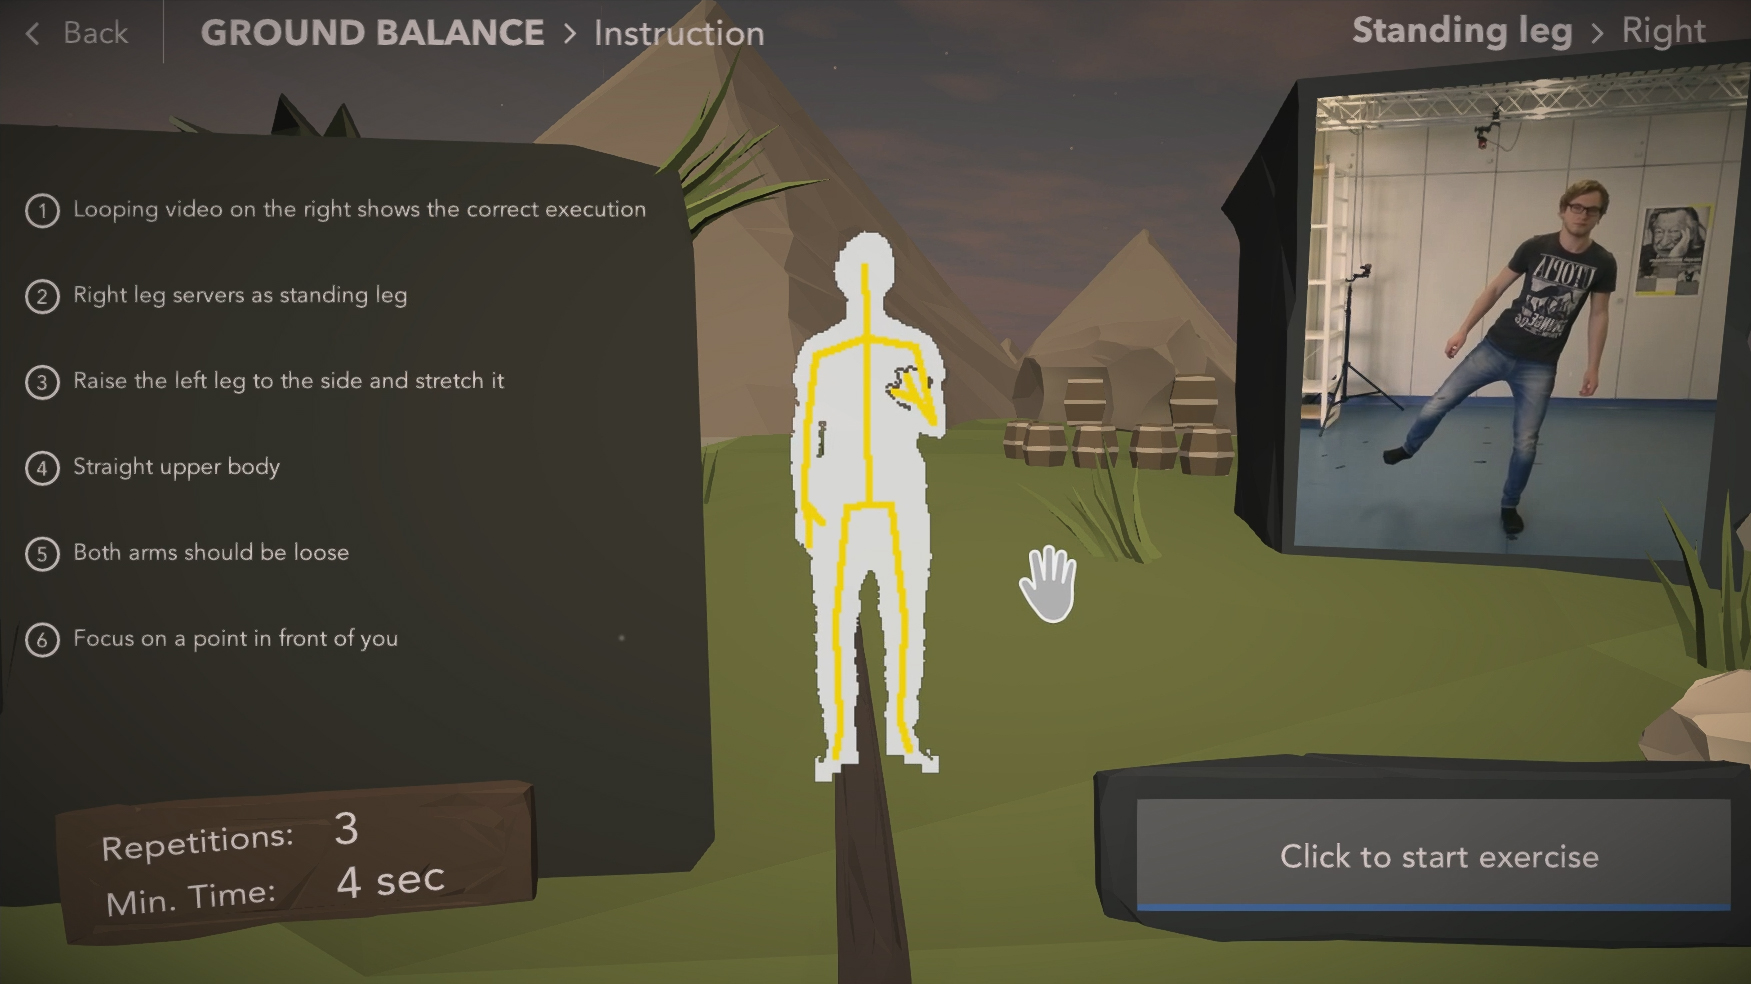
\includegraphics[width=1\linewidth]{Pictures/5_Workflow/10_ExerciseInstruction}
		\subcaption{Instruction into an exercise}%
		\label{fig:5_3_exercise_intro}
	\end{minipage}
	\caption{Instruction screens for a level and an exercises}%
	\label{fig:5_3_introductions}
\end{figure}

\subsubsection{Exercise Execution}
The exercise execution consists of the biggest functionality implementation (Figure~\ref{fig:5_3_exercise_execution}). Feedback indicators provide the user with necessary information about the current exercise in real time. This should help to enhance the performance in her execution and for successfully accomplishing the exercise. In the SLS the following feedback indicators are integrated:

\begin{itemize}
\item Checklist about key elements of an exercise
\item Amount of repetitions in general, finished, and left
\item Correct performance of an exercise (Timer starts and confidence increases)
\item Elapsed time the user is performing the exercise (Timer with a filling circle)
\item How good the exercise is currently performed (Confidence/Progress bar)
\item If a repetition was successful (Audio signal, timer color, success text, and incrementing repetitions counter)
\item If a repetition attempt was not successful (Audio signal and timer reset)
\end{itemize}

\begin{comment}
\begin{itemize}
\item Checklist about key elements of an exercise (Small red cross if not in correct position or green checkmark if in correct position)
\item Amount of repetitions in general, finished, and left
\item Correct performance of an exercise (Timer starts and confidence begins to increase)
\item Elapsed time the user is performing the exercise (Big timer with a filling circle around it)
\item How good or far the exercise is currently performed (Blue confidence/progress bar)
\item If the repetition was successful (Audio signal, timer changes color to green, success text, and incrementing repetitions counter)
\item If a repetition attempt was not successful (Audio signal and timer reset)
\end{itemize}

\end{comment}

After each successful exercise execution the user is forwarded to a summary screen (Figure~\ref{fig:5_3_exercise_summary}).
She gets an overview about performance parameters for the execution time, attempts, and the confidence for each repetition. Averaged values for the accomplished side summarize this.
%A similar summary screen exists for the entire level if all exercises of it have been accomplished. The same parameters are given but averaged (Figure~\ref{fig:5_3_level_summary}).
A similar summary screen for the entire level can be selected in the exercise menu. It provides an overview of the same performance parameters for each exercise in average (Figure~\ref{fig:5_3_level_summary}).

\begin{comment}
\item When an exercise is currently correctly performed
\item How good the exercise is currently performed, namely the confidence
\item The elapsed time the user is performing the exercise
\item When the repetition is successfully accomplished, i.e. the minimum time has been reached
\item When an repetition attempt was not successful
\item How many repetitions in general, finished and left
\item Checklist about key elements in an execution (like hands up, foot stretched, etc.)
\item A summary that shows the user parameters about the performance (execution time, overall attempts, confidence) for each repetition and an average value of these
\item A similar summary can also be found for the entire stage, where the same parameters for each exercise are listed in average
\end{comment}

\begin{figure}[htb]
	\centering
	\begin{minipage}[t]{1\linewidth}
		\centering
		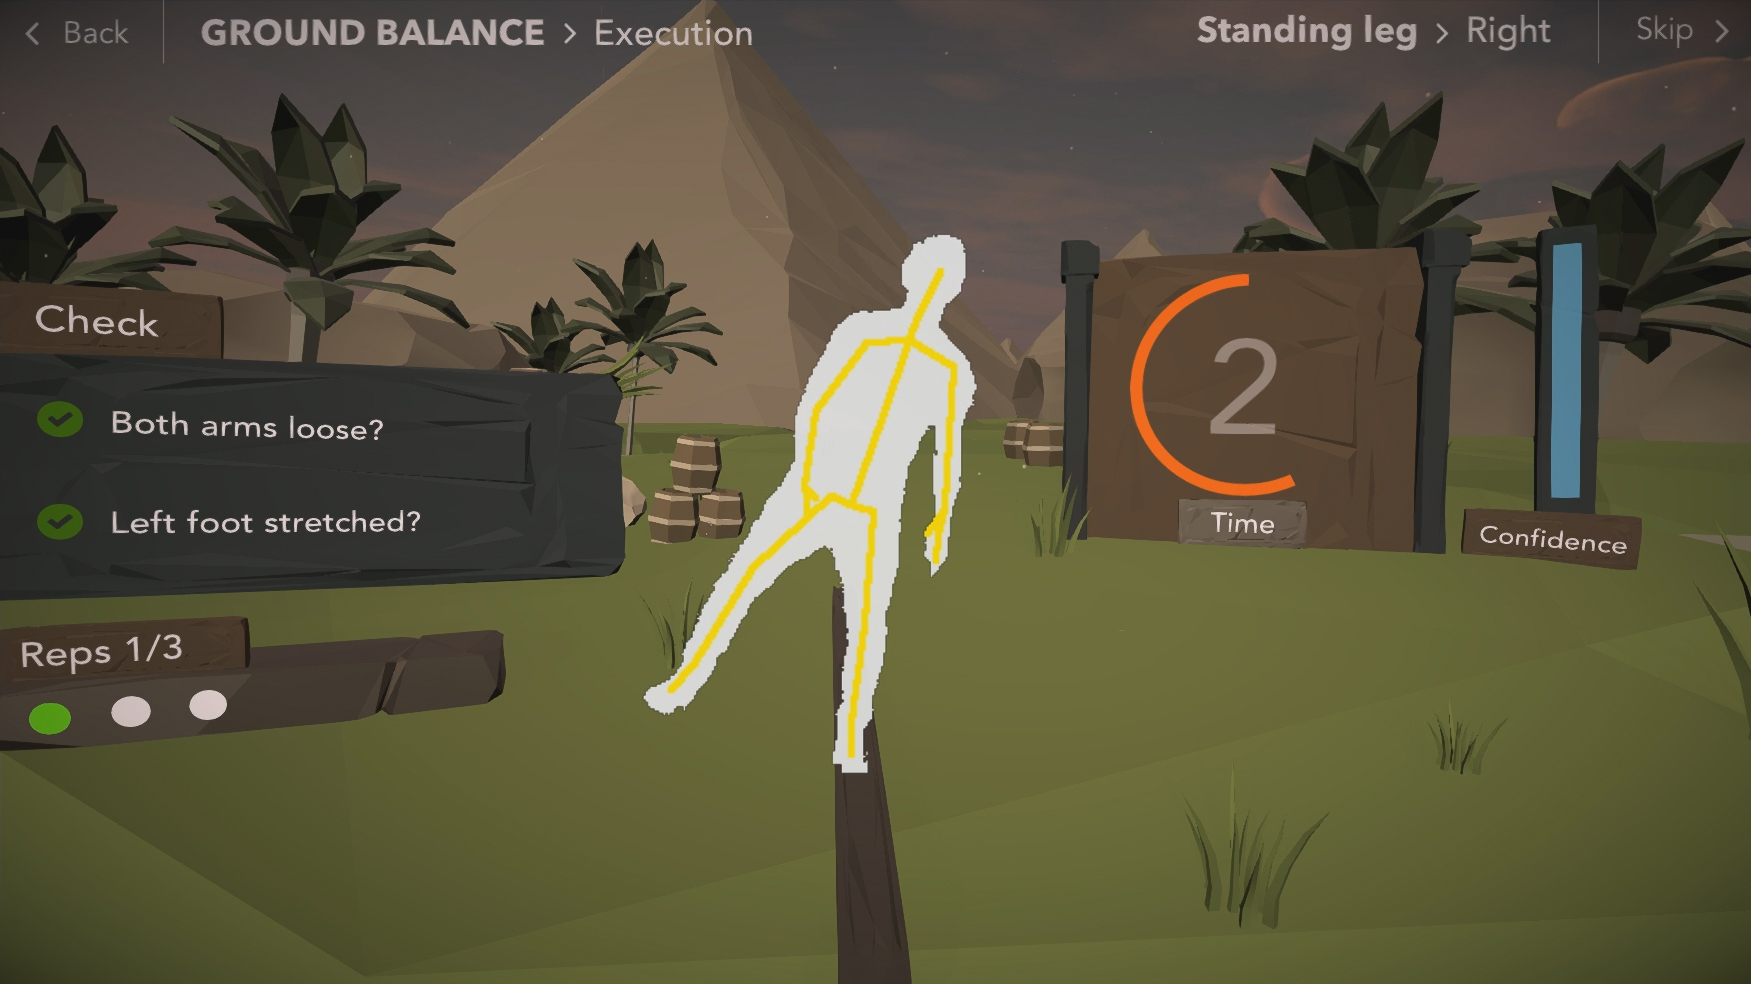
\includegraphics[width=0.57\linewidth]{Pictures/5_Workflow/11_3_ExerciseExecutionRep}
		\subcaption{Exercise execution}
		\label{fig:5_3_exercise_execution}
	\end{minipage}
	\hfill
	\begin{minipage}[t]{0.49\linewidth}
		\centering
		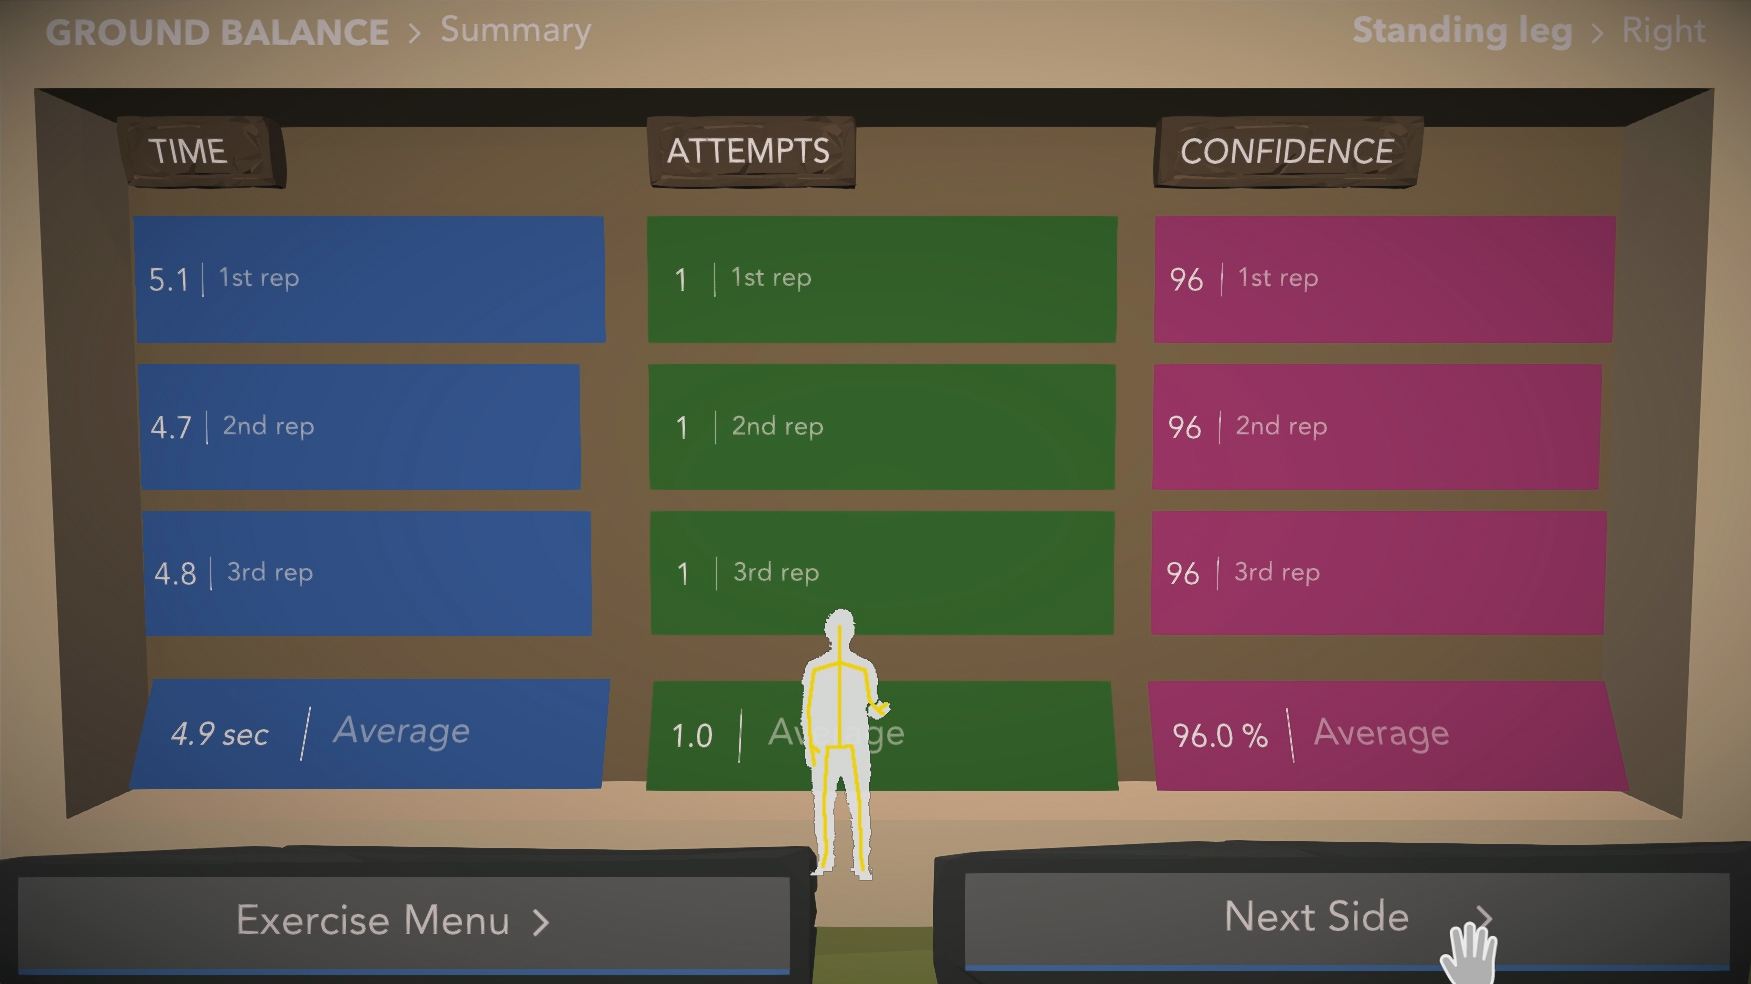
\includegraphics[width=1\linewidth]{Pictures/5_Workflow/12_ExerciseSummary}
		\subcaption{Exercise summary}
		\label{fig:5_3_exercise_summary}
	\end{minipage}
	\hfill
	\begin{minipage}[t]{0.49\linewidth}
		\centering
		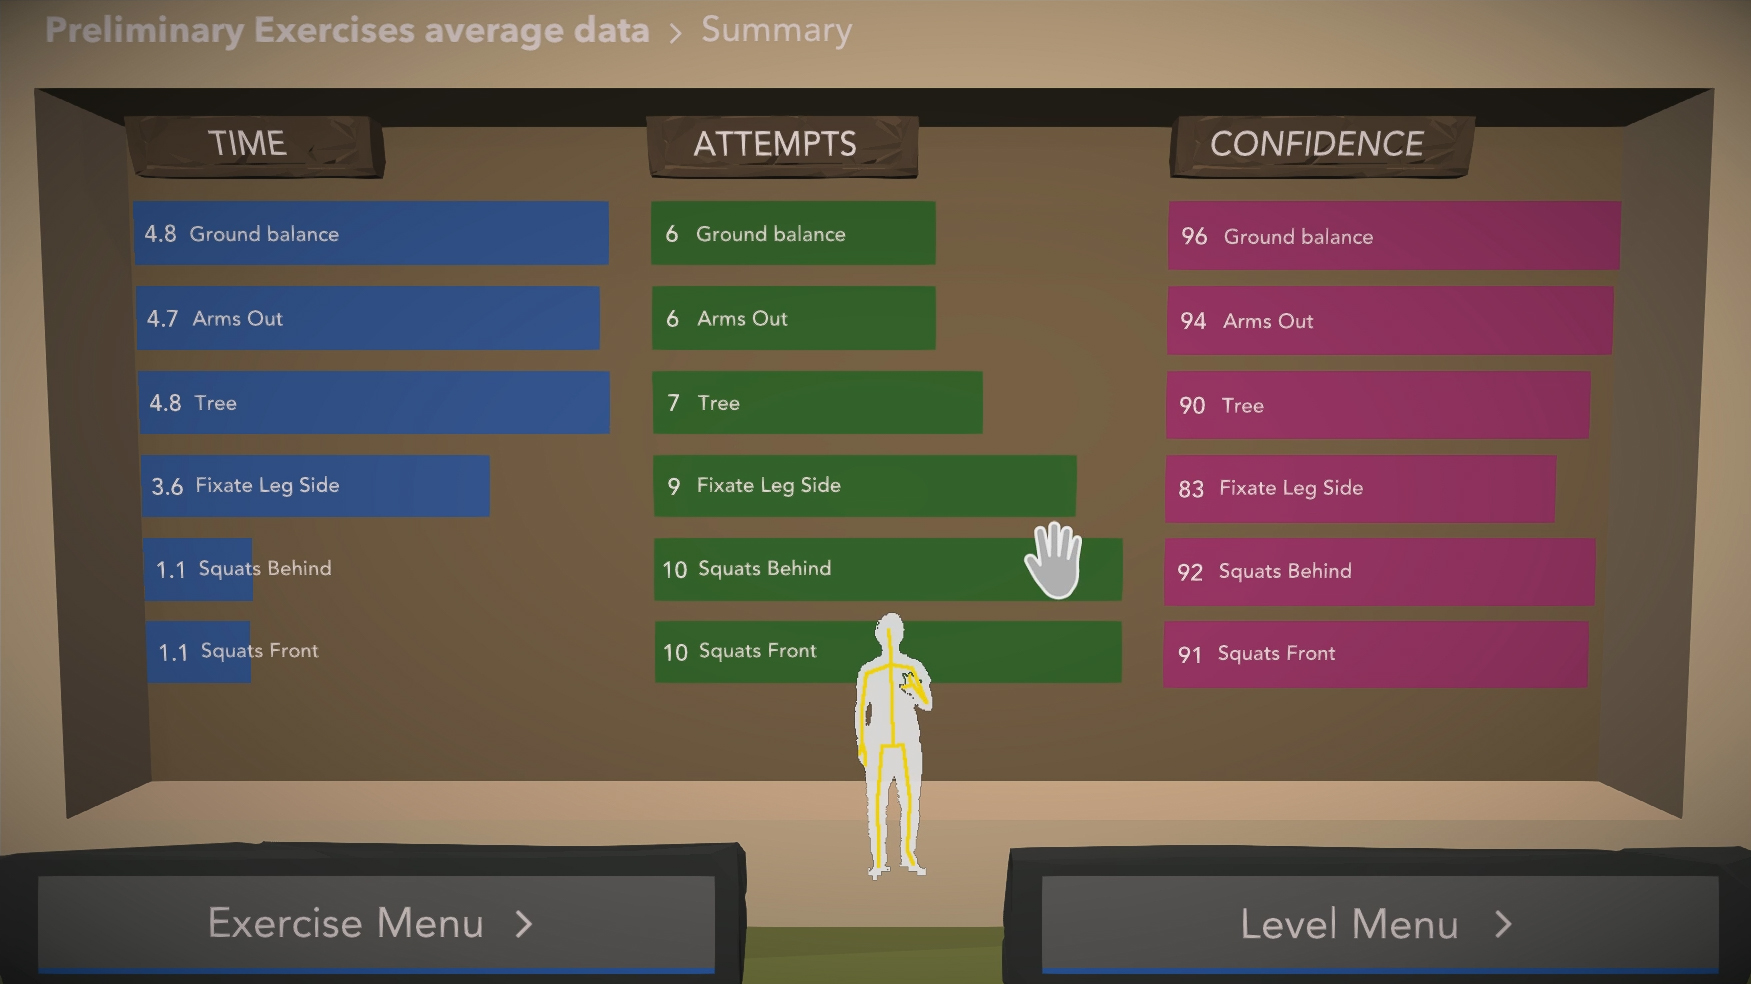
\includegraphics[width=1\linewidth]{Pictures/5_Workflow/13_TierSummary}
		\subcaption{Level summary}
		\label{fig:5_3_level_summary}
	\end{minipage}
	\caption{Exercise execution and summary screens}
	\label{fig:5_3_exercise_sequence}
\end{figure}
